%!TEX root = main.tex

\documentclass[letterpaper, 10 pt, conference]{ieeeconf}  % Comment this line out if you need a4paper
\IEEEoverridecommandlockouts                              % This command is only needed if 
                                                          % you want to use the \thanks command
\overrideIEEEmargins                                      % Needed to meet printer requirements.

% Default packages

\usepackage{graphicx}
\graphicspath{{images/}}
% \usepackage{amsmath} % Commented because it's added later with an option (under Tommy's packages)

\usepackage{color}
\usepackage[dvipsnames]{xcolor}
\usepackage{booktabs}
\usepackage{textcomp}
\usepackage{subcaption}
% Some optional stuff you might like/need.
\usepackage{microtype} % Improved Tracking and Kerning
% \usepackage[all]{hypcap}  % Fixes bug in hyperref caption linking
\usepackage{hyperref}
\usepackage{ccicons}  % Cite your images correctly!
% \usepackage[utf8]{inputenc} % for a UTF8 editor only

% Macro space after
\usepackage{xspace}

\usepackage{tabularx}
\usepackage[labelfont=bf,font=footnotesize]{caption}
\usepackage{amssymb}
\usepackage{multirow}
\usepackage{verbatim}
% Fancy table stuff
\usepackage{booktabs}
\newcommand{\ra}[1]{\renewcommand{\arraystretch}{#1}}
\renewcommand{\baselinestretch}{0.97}

% Macros
\newcommand{\todo}[1]{\textcolor{blue}{#1}}
\newcommand{\repword}[1]{\textcolor{red}{#1}}
\newcommand{\question}[1]{\textcolor{OliveGreen}{\textbf{#1}}}
\newcommand{\iffy}[1]{\textcolor{OliveGreen}{#1}}
\newcommand{\Bezier}{B\'{e}zier\xspace}
\newcommand{\plucker}{Pl\"{u}cker\xspace}

% Useful stylized abbreviations
\makeatletter
\DeclareRobustCommand\onedot{\futurelet\@let@token\@onedot}
\def\@onedot{\ifx\@let@token.\else.\null\fi\xspace}

\def\eg{\emph{e.g}\onedot} \def\Eg{\emph{E.g}\onedot}
\def\ie{\emph{i.e}\onedot} \def\Ie{\emph{I.e}\onedot}
\def\cf{\emph{c.f}\onedot} \def\Cf{\emph{C.f}\onedot}
\def\etc{\emph{etc}\onedot} \def\vs{\emph{vs}\onedot}
\def\wrt{w.r.t\onedot} \def\dof{d.o.f\onedot}
\def\etal{\emph{et al}\onedot}
\makeatother

% Lorem
\usepackage{lipsum}

% Fix for package enumitem
\let\labelindent\relax

% Place figures at the bottom of a page
\usepackage{dblfloatfix}

% Tommy's packages
\usepackage[utf8]{inputenc}
\usepackage[intlimits]{amsmath}
\usepackage{amsfonts}
\usepackage{amssymb}
\usepackage{ragged2e}
\usepackage[letterpaper, margin=1in]{geometry}
\usepackage{graphicx}
\usepackage{cancel}
\usepackage{mathtools}
\usepackage{tabularx}
\usepackage{arydshln}
\usepackage{tensor}
\usepackage{array}
\usepackage{xcolor}
\usepackage[boxed]{algorithm}
\usepackage[noend]{algpseudocode}
\usepackage{listings}
\usepackage{textcomp}
\usepackage{mathrsfs}
\usepackage{bbm}
\usepackage{tikz}
\usepackage{enumitem}
\usepackage{arydshln}
\usepackage{relsize}
\usepackage{multicol}

\usetikzlibrary{bayesnet}

% Thanks Jana!
\lstdefinestyle{custompy}{
  belowcaptionskip=1\baselineskip,
  breaklines=true,
  xleftmargin=\parindent,
  language=Python,
  showstringspaces=false,
  basicstyle=\footnotesize\ttfamily,
  keywordstyle=\bfseries\color{green!40!black},
  commentstyle=\itshape\color{purple!40!black},
  identifierstyle=\color{blue},
  stringstyle=\color{orange},
}

% %%%%%%%%%%%%%%%%%%%%%%%%%%%%%%%%%%%%%%%%%%%%%%%%%%%%%%%%%%%%%%%%%%%%%%%%%%%%%%%%%%%%%
%
% End packages
%
% %%%%%%%%%%%%%%%%%%%%%%%%%%%%%%%%%%%%%%%%%%%%%%%%%%%%%%%%%%%%%%%%%%%%%%%%%%%%%%%%%%%%%

%%%%%%%%%%%%%%%%%%%%%%%%%%%%%
% Formatting commands
%%%%%%%%%%%%%%%%%%%%%%%%%%%%%
\newcommand{\n}{\hfill\break}
\newcommand{\up}{\vspace{-\baselineskip}}
\newcommand{\hangblock}[2]{\par\noindent\settowidth{\hangindent}{\textbf{#1: }}\textbf{#1: }\!\!\!#2}
\newcommand{\lemma}[1]{\hangblock{Lemma}{#1}}
\newcommand{\defn}[1]{\hangblock{Defn}{#1}}
\newcommand{\thm}[1]{\hangblock{Thm}{#1}}
\newcommand{\cor}[1]{\hangblock{Cor}{#1}}
\newcommand{\prop}[1]{\hangblock{Prop}{#1}}
\newcommand{\ex}[1]{\hangblock{Ex}{#1}}
\newcommand{\exer}[1]{\hangblock{Exer}{#1}}
\newcommand{\fact}[1]{\hangblock{Fact}{#1}}
\newcommand{\remark}[1]{\hangblock{Remark}{#1}}
\newcommand{\proven}{\;$\square$\n}
\newcommand{\problem}[1]{\par\noindent{#1}\n}
\newcommand{\problempart}[2]{\par\noindent\indent{}\settowidth{\hangindent}{\textbf{(#1)} \indent{}}\textbf{(#1)} #2\n}
\newcommand{\ptxt}[1]{\textrm{\textnormal{#1}}}
\newcommand{\inlineeq}[1]{\centerline{$\displaystyle #1$}}
\newcommand{\pageline}{\noindent\rule{\textwidth}{0.1pt}}

%%%%%%%%%%%%%%%%%%%%%%%%%%%%%
% Math commands
%%%%%%%%%%%%%%%%%%%%%%%%%%%%%
% Set Theory
\newcommand{\card}[1]{\left|#1\right|}
\newcommand{\set}[1]{\left\{#1\right\}}
\newcommand{\setmid}{\;\middle|\;}
\newcommand{\ps}[1]{\mathcal{P}\left(#1\right)}
\newcommand{\pfinite}[1]{\mathcal{P}^{\ptxt{finite}}\left(#1\right)}
\newcommand{\naturals}{\mathbb{N}}
\newcommand{\N}{\naturals}
\newcommand{\integers}{\mathbb{Z}}
\newcommand{\Z}{\integers}
\newcommand{\rationals}{\mathbb{Q}}
\newcommand{\Q}{\rationals}
\newcommand{\reals}{\mathbb{R}}
\newcommand{\R}{\reals}
\newcommand{\complex}{\mathbb{C}}
\newcommand{\C}{\complex}
\newcommand{\halfPlane}{\mathbb{H}}
\let\H\relax
\newcommand{\H}{\halfPlane}
\newcommand{\comp}{^{\complement}}
\DeclareMathOperator{\Hom}{Hom}
\newcommand{\Ind}{\mathbbm{1}}
\newcommand{\cut}{\setminus}
\DeclareMathOperator{\elem}{elem}

% Graph Theory
\let\deg\relax
\DeclareMathOperator{\deg}{deg}
\newcommand{\degp}{\ptxt{deg}^{+}}
\newcommand{\degn}{\ptxt{deg}^{-}}
\newcommand{\precdot}{\mathrel{\ooalign{$\prec$\cr\hidewidth\hbox{$\cdot\mkern0.5mu$}\cr}}}
\newcommand{\succdot}{\mathrel{\ooalign{$\cdot\mkern0.5mu$\cr\hidewidth\hbox{$\succ$}\cr\phantom{$\succ$}}}}
\DeclareMathOperator{\cl}{cl}
\DeclareMathOperator{\affdim}{affdim}

% Probability
\newcommand{\parSymbol}{\P}
\newcommand{\Prob}{\mathbb{P}}
\renewcommand{\P}{\Prob}
\newcommand{\Avg}{\mathbb{E}}
\newcommand{\E}{\Avg}
\DeclareMathOperator{\Var}{Var}
\DeclareMathOperator{\cov}{cov}
\DeclareMathOperator{\Unif}{Unif}
\DeclareMathOperator{\Binom}{Binom}
\newcommand{\CI}{\mathrel{\text{\scalebox{1.07}{$\perp\mkern-10mu\perp$}}}}

% Standard Math
\newcommand{\inv}{^{-1}}
\newcommand{\abs}[1]{\left|#1\right|}
\newcommand{\ceil}[1]{\left\lceil{}#1\right\rceil{}}
\newcommand{\floor}[1]{\left\lfloor{}#1\right\rfloor{}}
\newcommand{\conj}[1]{\overline{#1}}
\newcommand{\of}{\circ}
\newcommand{\tri}{\triangle}
\newcommand{\inj}{\hookrightarrow}
\newcommand{\surj}{\twoheadrightarrow}
\newcommand{\ndiv}{\nmid}
\renewcommand{\epsilon}{\varepsilon}
\newcommand{\divides}{\mid}
\newcommand{\ndivides}{\nmid}
\DeclareMathOperator{\lcm}{lcm}
\DeclareMathOperator{\sgn}{sgn}
\newcommand{\map}[4]{\!\!\!\begin{array}[t]{rcl}#1 & \!\!\!\!\to & \!\!\!\!#2\\ #3 & \!\!\!\!\mapsto & \!\!\!\!#4\end{array}}
\newcommand{\bigsum}[2]{\smashoperator[lr]{\sum_{\scalebox{#1}{$#2$}}}}

% Linear Algebra
\newcommand{\Id}{\textrm{\textnormal{Id}}}
\newcommand{\im}{\textrm{\textnormal{im}}}
\newcommand{\norm}[1]{\abs{\abs{#1}}}
\newcommand{\tpose}{^{T}\!}
\newcommand{\iprod}[1]{\left<#1\right>}
\DeclareMathOperator{\tr}{tr}
\DeclareMathOperator{\trace}{tr}
\newcommand{\chgBasMat}[3]{\!\!\tensor*[_{#1}]{\left[#2\right]}{_{#3}}}
\newcommand{\vecBas}[2]{\tensor*[]{\left[#1\right]}{_{#2}}}
\DeclareMathOperator{\GL}{GL}
\DeclareMathOperator{\Mat}{Mat}
\DeclareMathOperator{\vspan}{span}
\DeclareMathOperator{\rank}{rank}
\newcommand{\V}[1]{\vec{#1}}
\DeclareMathOperator{\proj}{proj}
\DeclareMathOperator{\compProj}{comp}
\DeclareMathOperator{\row}{row}
\newcommand{\smallPMatrix}[1]{\paren{\begin{smallmatrix}#1\end{smallmatrix}}}
\newcommand{\smallBMatrix}[1]{\brack{\begin{smallmatrix}#1\end{smallmatrix}}}
\newcommand{\pmat}[1]{\begin{pmatrix}#1\end{pmatrix}}
\newcommand{\bmat}[1]{\begin{bmatrix}#1\end{bmatrix}}

% Multilinear Algebra
\newcommand{\Lsym}{\L}
\let\L\relax
\DeclareMathOperator{\L}{\mathscr{L}}
\DeclareMathOperator{\A}{\mathcal{A}}
\DeclareMathOperator{\Alt}{Alt}
\DeclareMathOperator{\Sym}{Sym}
\newcommand{\ot}{\otimes}
\newcommand{\ox}{\otimes}
\DeclareMathOperator{\asc}{asc}
\DeclareMathOperator{\asSet}{set}
\DeclareMathOperator{\sort}{sort}
\DeclareMathOperator{\ringA}{\mathring{A}}

% Topology
\newcommand{\closure}[1]{\overline{#1}}
\newcommand{\uball}{\mathcal{U}}
\DeclareMathOperator{\Int}{Int}
\DeclareMathOperator{\Ext}{Ext}
\DeclareMathOperator{\Bd}{Bd}
\DeclareMathOperator{\rInt}{rInt}
\DeclareMathOperator{\ch}{ch}
\DeclareMathOperator{\ah}{ah}
\newcommand{\LargerTau}{\mathlarger{\mathlarger{\mathlarger{\mathlarger{\tau}}}}}
\newcommand{\Tau}{\mathcal{T}}

% Analysis
\DeclareMathOperator{\Graph}{Graph}
\DeclareMathOperator{\epi}{epi}
\DeclareMathOperator{\hypo}{hypo}
\DeclareMathOperator{\supp}{supp}
\newcommand{\lint}[2]{\underset{#1}{\overset{#2}{{\color{black}\underline{{\color{white}\overline{{\color{black}\int}}\color{black}}}}}}}
\newcommand{\uint}[2]{\underset{#1}{\overset{#2}{{\color{white}\underline{{\color{black}\overline{{\color{black}\int}}\color{black}}}}}}}
\newcommand{\alignint}[2]{\underset{#1}{\overset{#2}{{\color{white}\underline{{\color{white}\overline{{\color{black}\int}}\color{black}}}}}}}
\newcommand{\extint}{\ptxt{ext}\int}
\newcommand{\extalignint}[2]{\ptxt{ext}\alignint{#1}{#2}}
\newcommand{\conv}{\ast}
\newcommand{\pd}[2]{\frac{\partial{}#1}{\partial{}#2}}
\newcommand{\del}{\nabla}
\DeclareMathOperator{\grad}{grad}
\DeclareMathOperator{\curl}{curl}
\let\div\relax
\DeclareMathOperator{\div}{div}
\DeclareMathOperator{\vol}{vol}

% Complex Analysis
\let\Re\relax
\DeclareMathOperator{\Re}{Re}
\let\Im\relax
\DeclareMathOperator{\Im}{Im}
\DeclareMathOperator{\Res}{Res}

% Abstract Algebra
\DeclareMathOperator{\ord}{ord}
\newcommand{\generated}[1]{\left<#1\right>}
\newcommand{\cycle}[1]{\smallPMatrix{#1}}
\newcommand{\id}{\ptxt{id}}
\newcommand{\iso}{\cong}
\DeclareMathOperator{\Aut}{Aut}
\DeclareMathOperator{\SL}{SL}
\DeclareMathOperator{\op}{op}
\newcommand{\isom}[4]{\!\!\!\begin{array}[t]{rcl}#1 & \!\!\!\!\overset{\sim}{\to} & \!\!\!\!#2\\ #3 & \!\!\!\!\mapsto & \!\!\!\!#4\end{array}}
\newcommand{\F}{\mathbb{F}}
\newcommand{\acts}{\;\rotatebox[origin=c]{-90}{$\circlearrowright$}\;}
\newcommand{\disjunion}{\mathrel{\text{\scalebox{1.07}{$\perp\mkern-10mu\perp$}}}}
\DeclareMathOperator{\SO}{SO}
\DeclareMathOperator{\stab}{stab}
\DeclareMathOperator{\nullity}{nullity}

% Convex Optimization
\newcommand{\sectionSymbol}{\S}
\let\S\relax
\newcommand{\S}{\mathbb{S}}
\DeclareMathOperator{\dist}{dist}
\DeclareMathOperator{\dom}{dom}
\DeclareMathOperator{\diag}{diag}
\DeclareMathOperator{\ones}{\mathbbm{1}}
\newcommand{\minimizeOver}[3]{\begin{array}{rl}\underset{#1}{\ptxt{minimize}} & #2\\ \ptxt{subject to} & #3\end{array}}
\newcommand{\maximizeOver}[3]{\begin{array}{rl}\underset{#1}{\ptxt{maximize}} & #2\\ \ptxt{subject to} & #3\end{array}}
\newcommand{\minimizationProblem}[2]{\minimizeOver{}{#1}{#2}}
\newcommand{\maximizationProblem}[2]{\maximizeOver{}{#1}{#2}}

% Proofs
\newcommand{\st}{s.t.}
\newcommand{\unique}{!}
\newcommand{\iffdef}{\overset{\ptxt{def}}{\Leftrightarrow}}
\newcommand{\eqdef}{\overset{\ptxt{def}}{=}}
\newcommand{\eqVertical}{\rotatebox[origin=c]{90}{=}}
\newcommand{\mapsfrom}{\mathrel{\reflectbox{\ensuremath{\mapsto}}}}
\newcommand{\mapsdown}{\rotatebox[origin=c]{-90}{$\mapsto$}\mkern2mu}
\newcommand{\mapsup}{\rotatebox[origin=c]{90}{$\mapsto$}\mkern2mu}
\newcommand{\from}{\!\mathrel{\reflectbox{\ensuremath{\to}}}}

% Brackets
\newcommand{\paren}[1]{\left(#1\right)}
\renewcommand{\brack}[1]{\left[#1\right]}
\renewcommand{\brace}[1]{\left\{#1\right\}}
\newcommand{\ang}[1]{\left<#1\right>}

% Algorithms
\algrenewcommand{\algorithmiccomment}[1]{\hskip 1em \texttt{// #1}}
\algrenewcommand\algorithmicrequire{\textbf{Input:}}
\algrenewcommand\algorithmicensure{\textbf{Output:}}
\newcommand{\algP}{\ptxt{\textbf{P}}}
\newcommand{\algNP}{\ptxt{\textbf{NP}}}
\newcommand{\algNPC}{\ptxt{\textbf{NP-Complete}}}
\newcommand{\algNPH}{\ptxt{\textbf{NP-Hard}}}
\newcommand{\algEXP}{\ptxt{\textbf{EXP}}}

%%%%%%%%%%%%%%%%%%%%%%%%%%%%%
% Other commands
%%%%%%%%%%%%%%%%%%%%%%%%%%%%%
\newcommand{\flag}[1]{\textbf{\textcolor{red}{#1}}}
\newcommand{\uSym}{\u}
\let\u\relax
\newcommand{\u}[1]{\underline{#1}}
\newcommand{\bSym}{\b}
\let\b\relax
\newcommand{\b}[1]{\textbf{#1}}
\newcommand{\iSym}{\i}
\let\i\relax
\newcommand{\i}[1]{\textit{#1}}

%%%%%%%%%%%%%%%%%%%%%%%%%%%%%%%%%%%%%%%
% Make l's curvy in math environments %
%%%%%%%%%%%%%%%%%%%%%%%%%%%%%%%%%%%%%%%
\mathcode`l="8000
\begingroup
\makeatletter
\lccode`\~=`\l
\DeclareMathSymbol{\lsb@l}{\mathalpha}{letters}{`l}
\lowercase{\gdef~{\ifnum\the\mathgroup=\m@ne \ell \else \lsb@l \fi}}%
\endgroup

%%%%%%%%%%%%%%%%%%%%%%%%%
% Fix \vdots and \ddots %
%%%%%%%%%%%%%%%%%%%%%%%%%
\usepackage{letltxmacro}
\LetLtxMacro\orgvdots\vdots
\LetLtxMacro\orgddots\ddots

\makeatletter
\DeclareRobustCommand\vdots{%
  \mathpalette\@vdots{}%
}
\newcommand*{\@vdots}[2]{%
  % #1: math style
  % #2: unused
  \sbox0{$#1\cdotp\cdotp\cdotp\m@th$}%
  \sbox2{$#1.\m@th$}%
  \vbox{%
    \dimen@=\wd0 %
    \advance\dimen@ -3\ht2 %
    \kern.5\dimen@
    % remove side bearings
    \dimen@=\wd2 %
    \advance\dimen@ -\ht2 %
    \dimen2=\wd0 %
    \advance\dimen2 -\dimen@
    \vbox to \dimen2{%
      \offinterlineskip
      \copy2 \vfill\copy2 \vfill\copy2 %
    }%
  }%
}
\DeclareRobustCommand\ddots{%
  \mathinner{%
    \mathpalette\@ddots{}%
    \mkern\thinmuskip
  }%
}
\newcommand*{\@ddots}[2]{%
  % #1: math style
  % #2: unused
  \sbox0{$#1\cdotp\cdotp\cdotp\m@th$}%
  \sbox2{$#1.\m@th$}%
  \vbox{%
    \dimen@=\wd0 %
    \advance\dimen@ -3\ht2 %
    \kern.5\dimen@
    % remove side bearings
    \dimen@=\wd2 %
    \advance\dimen@ -\ht2 %
    \dimen2=\wd0 %
    \advance\dimen2 -\dimen@
    \vbox to \dimen2{%
      \offinterlineskip
      \hbox{$#1\mathpunct{.}\m@th$}%
      \vfill
      \hbox{$#1\mathpunct{\kern\wd2}\mathpunct{.}\m@th$}%
      \vfill
      \hbox{$#1\mathpunct{\kern\wd2}\mathpunct{\kern\wd2}\mathpunct{.}\m@th$}%
    }%
  }%
}
\makeatother

\newcommand{\B}{
  
\begin{tikzpicture}
  \filldraw [fill=red, draw=black] (0, 0) rectangle (0.37, 0.45);
  \draw [line width=0.5mm, white ] (0.1,0.08) -- (0.1,0.38);
  \draw[line width=0.5mm, white ] (0.1, 0.35) .. controls (0.2, 0.35) and (0.4, 0.2625) .. (0.1, 0.225);
  \draw[line width=0.5mm, white ] (0.1, 0.225) .. controls (0.2, 0.225) and (0.4, 0.1625) .. (0.1, 0.1);
  \end{tikzpicture}
}

% --------------------------------------------------- 
%                    Title & Authors
% --------------------------------------------------- 

\title{Predictive Statistical Modeling of Atlantic Hurricanes}

\author{Thomas Cohn}


\usepackage[style=mla-new]{biblatex}
\addbibresource{ref.bib}


% --------------------------------------------------- 
%                    Document
% --------------------------------------------------- 

\begin{document}

\maketitle
\thispagestyle{plain}
\pagestyle{plain}

\section{Introduction}
%!TEX root = ../main.tex

\par
A hurricane is one of the most destructive weather events in the United States.
Every fall, major storms threaten states along the Gulf Coast and Atlantic ocean with high winds, heavy rain, and storm surge.
Some hurricanes proceed to make landfall, causing significant damage to life and property, while others avoid land altogether, having almost zero human impact.
So understandably, the modeling and prediction of Atlantic hurricanes is an important topic of study.

\par
I will begin by attempting to describe an accurate probability distribution for the number of tropical storms in a given year, and the number of landfalling storms. We will consider both multiple parametric distributions, and compare to a nonparametric distribution.
Next, I will compare several methods for predicting whether a hurricane will make landfall, and under what circumstances, based on information from the formation and early life of the storm.
Finally, I will examine the frequency of outlier hurricanes, to analyze how common unexpected or unpredicted events are.

% \section{Related Work}
% %!TEX root = ../main.tex

In their paper \textit{Manifold Learning for Multivariate Variable-Length Sequences With an Application to Similarity Search},~\cite{ho2015manifold} present several similarity measures for variable length data sequences, and apply them to manifold learning on Hurricanes.
This will provide the basis for one of our predictive methods for the path a hurricane will take, and whether or not it will make landfall.

\section{Data}
%!TEX root = ../main.tex

\par
After an Atlantic hurricane dissipates, the National Hurricane Center (NHC) determines the most accurate track of the storm, and collects various other information about the storm throughout its lifetime.
The data is available online as a comma-separated values file.
The available data includes information about the hurricane taken every six hours, from the formation of the storm to its dissipation.
This includes:
\begin{itemize}
	\item Latitude and longitude of the system center
	\item Landfall events
	\item Maximum sustained wind
	\item Minimum barometric pressure
	\item Maximum extent of hurricane and tropical storm winds
\end{itemize}

\par
The tracked latitude and longitude of the system center is one very important component of the dataset, as it allows us to examine the path a hurricane has taken throughout its lifetime.
It also implicity gives us information on where the hurricane formed, and can be used to compare different storms to see how similar they are.

\par
The maximum sustained wind and minimum batrometric pressure are another useful piece of information to track.
Both represent the peak strength of a hurricane at a given time, albeit in different ways.
Maximum sustained wind speed and minimum barometric pressure are direct measurements of the power of a storm.
In addition, the change in barometric pressure indicates whether a storm is strengthening or weakening.
% https://www.rhinobldg.com/understanding-barometric-pressure-in-hurricanes/

\par
Finally, tracking whether or not a hurricane made landfall, and the conditions when it made landfall, allows us to esimate how dangerous the hurricane was.
A strong hurricane which never makes landfall is much less hazardous than a weak hurricane that does.
This also allows us to make larger judgements as to the number of damaging hurricanes per year.

\begin{figure}
	\centering
	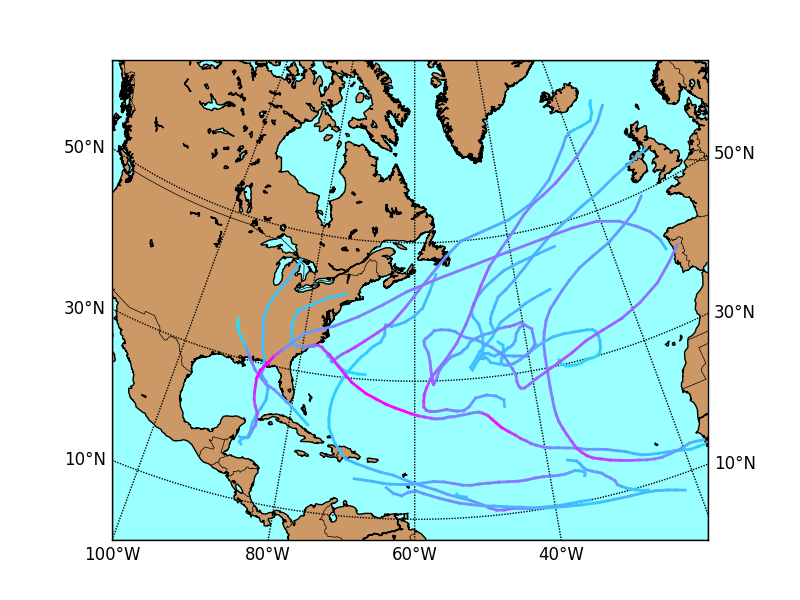
\includegraphics[width=\linewidth]{images/2018_max_winds.png}
	\caption{A map of the track of every Atlantic tropical storm in 2018. The color is scaled by the maximum wind speed.}
	\label{fig:2018_storm_tracks}
\end{figure}

\section{Method}
%!TEX root = ../main.tex

\subsection{Number of Storms}

\par
We will attempt to find the distributions which best fit the data on number of storms based on various loss functions.
Note that the number of landfalling storms is discrete.
The distributions I plan to examine include
\begin{itemize}
	\item Poisson
	\item Negative Binomial
\end{itemize}
For loss functions, I will examine common examples such as the 0-1 and quadratic loss functions, as well as defining some specific loss functions that make sense in the context of hurricanes.

\subsection{Predicting if a Storm will Make Landfall}

\subsection{Ourlier Analysis}

\section{Simulations}
%!TEX root = ../main.tex

\par
In order to generate more data from the limited real-world data available, I plan to add noise using various methods to existing data.
One method I will consider is simply adding Gaussian noise to each point in a track.
I will also generate random walks of the same length, and then add them pointwise to the hurricane.
I will analyze how realistic the data generated by these methods are, and use the larger dataset to examine the quality of my estimators.

\section{Analysis}
%!TEX root = ../main.tex

\par
I perform two major experiments to analyze the efficacy.
First, I need to determine the underlying dimensionality of the vector space the hurricanes lie in.
To do this, I try embedding a subset of the full dataset into $\R^{i}$ for $i=1,\ldots,15$, and then regressing the Nardaraya-Watson estimator for each case.
I then predict a different subset of the data to evaluate the accuracy of the model, for each number of dimensions.
In Figure ----, I plot the accuracy by the number of dimensions $i$.
In Figure ----, I plot the accuracy (but this time only including points for which the estimator has at least $90\%$ confidence) by the number of dimensions.
Since there's little improvement after $i=15$, I conclude that this is the optimal choice for the number of dimensions.

\begin{figure}
	\centering
	%\includegraphics[width=\linewidth]
	\caption{A plot of accuracy of the estimator versus the number of dimensions the hurricanes are embedded into by KPCA.}
	\label{fig:dimensions}
\end{figure}

\begin{figure}
	\centering
	%\includegraphics[width=\linewidth]
	\caption{A plot of accuracy of the estimator for only points in which it has high confidence (at least $90\%$) versus the number of dimensions the hurricanes are embedded into by KPCA.}
	\label{fig:confident_dimensions}
\end{figure}

\section{Discussion}
%!TEX root = ../main.tex

% \par
% This section will largely need to be written after I have results.

% \par
% I imagine that one major takeaway from my project will be the fact that historical and generated data alone don't do a great job of modeling hurricanes.
% I expect to see many outliers, and that the predictions may not be reliable to the degree needed for weather forecasting.
% The incorporation of weather models, and the inclusion of larger scale weather patterns such as El Ni\~{n}o, could likely provide much more accurate results, and would be an interesting direction for future research.

% \par
% I will also mention the fact that larger scale changes in weather patterns, due to global warming, may present some skew in the results.
% It would be helpful to take this into account while trying to fit probability distributions to hurricane data.

\par
In this paper, I've presented a new statistical method for predicting whether or not a hurricane will make landfall.
I use time series similarity metrics to compare hurricanes, and use KPCA to find a representation for them in a Euclidean space.
I then use Nardaraya-Watson kernel regression to approximate the relationship between these embedded coordinates and the probability a hurricane will make landfall.
The analysis section provides evidence supporting the efficacy of my method.

\par
Of course, this is a relatively primitive model, and there's a wealth of available information about a hurricane that I don't utilize.
Factors such as the size of a storm, the extent in various directions of its winds, the barometric pressure, and much more could help tune an extension of the model to be much more accurate.

\par
Another challenge my technique faces is speed.
Computing the similarity between large numbers of hurricanes becomes expensive very quickly.
The number of comparisons is $O(n^{2})$ for the number of hurricanes in the training dataset, and each comparison is $O(\mathscr{L}(A)\mathscr{L}(B))$, even when utilizing dynamic programming.
With more computational resources, it would be possible to train and test on larger datasets, and make full use of the simulation capabilities to generate new data.

\par
Another ineresting area for future research would be high level modeling of hurricane behavior.
This could be useful for further tweaking the simulation work, such as choosing a better mean and/or covariance.

\par
Obviously, only $70\%$ accuracy is not enough to make life-or-death predictions, and any purely statistical model will always be inferior to a more complex model that takes present weather patterns into account.
However, this paper makes it clear that there are merits to using statistical techniques to model and understand hurricanes.

\printbibliography

\end{document}
